% !Mode:: "TeX:UTF-8"
%!TEX program  = xelatex

\documentclass[bwprint]{gmcmthesis}
\usepackage[framemethod=TikZ]{mdframed}
\usepackage{longtable}
\usepackage{lineno,hyperref}
\usepackage{amsmath}
\usepackage{float}
\usepackage{graphicx}
\usepackage{subfigure}
\usepackage{caption}
\title{疫情背景下的周边游需求图谱分析}
\baominghao{4321} %参赛队号
\schoolname{XX大学}%学校名称
\membera{小米} %队员A
\memberb{向左} %队员B
\memberc{哈哈} %队员C
\begin{document}

 %生成标题
 \maketitle

 %填写摘要
\begin{abstract}
近年来,随着OTA与CTG文本数据的火爆,其中蕴含充分的文旅实体信息。针对问题一,本文构建LDA主题模型实现对微信公众号推文与游记攻略文本的分类,并结合主题词库,比较分类的高频主题词,实现了对文本数据的文旅 主题相关性识别。针对问题二,……………………。针对问题三,本文针对实体提取其Bert表征,并利用其作为图卷积神经网络的节点输入表征,随后利用图神经网络良好的高阶连接性,本文得到了旅游实体之间的相关性预测。针对问题四,本文对上述……………


\keywords{LDA模型\quad  Bert\quad 图神经网络}
\end{abstract}

\pagestyle{plain}

%目录 不推荐加
%\tableofcontents

\section{问题重述}

\subsection{引言}

近年来,基于文本形式的在线旅游与用户生成内容愈发成为人们获取旅游信息进行攻略查询的重要信息来源。在这些信息中,有许多内容蕴含丰富的旅游相关信息,比如各文旅实体可能之间存在某种内在联系能够通过一定手段被挖掘出来,进而能够用作数据分析、营销产品设计及推荐系统等业务。因此,从众多文本数据中筛选出与文旅主题相关的信息,进而运用知识图谱手段挖掘文旅实体之间内在联系具有重要意义。

\subsection{问题的提出}

\begin{itemize}
	\item 问题一:针对附件中的微信公众号推文和游记攻略子表,根据其中每条推文或攻略与文旅的相关度进行分类,将他们分为相关或是不相关。其中与文旅相关的高频主题词可能包括:旅游,活动,交通,酒店,景区,假期,游客,农家乐等。
 
	\item 问题二:根据附件中提供的对景区、酒店等旅游产品的评价,外加游记攻略和公众号推文,对其中蕴含的旅游实体进行识别和提取。随后对上述实体构建热度评价模型,提取出其中较为热门的旅游产品实体。
 
	\item 问题三:根据表格中的OTA、UGC数据,对旅游产品进行关联度分析,找出以景区、酒店、餐饮为核心的强关联模式。并在此基础上进行可视化分析。
 
	\item 问题四:基于历史数据,分析疫情前后旅游产品变化。
\end{itemize}


% \section{模型的假设}

% \begin{itemize}
% \item 忽略实际加工误差对设计的影响;
% \item 木条与圆桌面之间的交接处缝隙较小,可忽略;
% \item 钢筋强度足够大,不弯曲;
% \item 假设地面平整。
% \end{itemize}

% \section{符号说明}

% \begin{tabular}{cc}
%  \hline
%  \makebox[0.4\textwidth][c]{符号}	&  \makebox[0.5\textwidth][c]{意义} \\ \hline
%  D	    & 木条宽度(cm) \\ \hline
%  L	    & 木板长度(cm)  \\ \hline
%  W	    & 木板宽度(cm)  \\ \hline
%  N	    & 第n根木条  \\ \hline
%  T	    & 木条根数  \\ \hline
%  H	    & 桌子高度(cm)  \\ \hline
%  R	    & 桌子半径(cm)  \\ \hline
%  R	    & 桌子直径(cm)  \\ \hline
% \end{tabular}

\section{问题分析}

\subsection{问题一分析}
利用附件中提供的公众号推文和游记攻略,本文需要构建适当模型根据其与文旅主题的相关性进行样本的有效划分。

首先,公众号推文包含标题、发表时间和正文信息。经过初步观察,推文标题和正文中都包含相与文旅相关的主题词,但其中有些正文内容收到其本身是广告或图片的形式,导致其内容体现在正文文本上与文旅主题相关程度不高。针对这类数据的预处理直接影响后续文本分类模型的好坏。

其次,游记攻略相关信息包括城市、游记标题、发布时间、出发时间、出行天数、人物、费用及正文。经过初步观察,游记攻略的标题和正文蕴含着丰富文本信息,但其中同样存在一些不相关的内容需要甄别,这也对后续的分类模型带来一定的挑战。


\subsection{问题二分析}
针对旅游产品的提取,最直观的是通过酒店、餐厅和旅游景点的评论信息进行提取,但是经过初步观察发现,在游记攻略中也蕴含丰富的文旅实体信息,如果忽略游记攻略是不妥的,在此本文考虑使用无监督学习方法对攻略中可能存在的实体信息进行提取。对旅游产品进行特征工程,最直观的为旅游产品被提及的次数,但直考虑次数不能够客观反映游客对旅游产品的满意程度,故根据文本的情感分析同样是十分必要的。


% \begin{figure}[!h]
% \centering
% 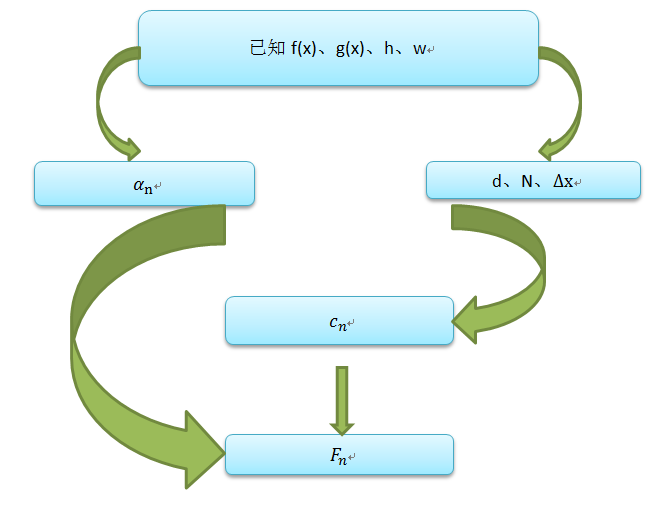
\includegraphics[width=.7\textwidth]{1.png}
% \caption{问题三流程图}
% \end{figure}

\subsection{问题三分析}
关联度构建可以考虑由公众号新闻和攻略出发进行挖掘,现有对图神经网络和知识图谱算法的研究十分热门,合理利用文本信息,挖掘其中关系,并在知识图谱火或是图神经网络中进行有效的高阶信息提取对于挖掘旅游产品之间关系十分重要。

\section{问题一建模与求解}

\subsection{数据预处理}

对于附件中给出的文本信息,由于前三问并不要求分析疫情前后文旅行业发生的变化,则首先应当将2018-2021年的数据进行合并。根据一定观察,发现公众号推文和游记的标题与正文都一定程度包含与文旅相关的内容,不能仅分析正文或是分析标题,故本文将标题与正文进行合并,用于后续的分析。

根据已经获得的文本信息,首先需要对其进行清理,将其中的数字、英文字母、特殊字符、换行符和空格等进行删除,这些信息对于基于中文的分析没有用处。对清理后的纯文本,对字段进行分词处理,方便随后进行进一步建模。

\subsection{模型构建与求解}

针对已有的文本,本文考虑构建LDA(Latent Dirichlet Allocation)主题模型实现文章与文旅相关性的划分在值得一提的是,在许多利用LDA模型进行主题分类的应用中,数据集的分布较为广泛,而考虑到本文数据集大部分与旅游是相关的,若在不引入外部数据集的情况下使用该模型,很可能分类效果不好。鉴于此,本文将LDA模型用作类似于K-means的聚类用途,根据其分类的文本特征再对文本主题进行分类。

LDA模型利用了贝叶斯的思想,将每个文本和每个主题词的先验分布均视为狄利克雷(Dirichlet)分布,其中文本词向量一致,目标是求语料库的分布。
\begin{gather}
	\theta_d \sim Dirichlet(\alpha) \\
	\beta_k \sim Dirichlet(\eta)
\end{gather}


其中随机变量$\theta_d$与$\beta_k$分别代表第$d$条文本和第$k$个主题词,$\alpha$和$\eta$分别代表分布的超参数向量,维度分别为$K$和$V$。对于第$d$条文本中的第$n$个词,根据多项分布可以得到其主题编号$z_{dn} \sim multi(\theta_d)$和词分布$w_{dn} \sim multi(\beta_{z_{dn}})$。则$(\alpha \rightarrow \theta_d \rightarrow z_d)$组成了Dirichlet-multi共轭分布。故能够得到$\theta_d$的后验分布$Dirichlet(\theta_d|\alpha + n_d)$,同样可以得到$\beta_k$的后验分布$Dirichlet(\beta_k|\eta + n_k)$。LDA模型的任务便是需要得到收敛的主题词$\beta$分布。至于LDA模型的求解,本文选用基于变分推断的EM算法。

要对文本进行基于文旅主题相关性的划分,首先要利用LDA模型进行文本主题划分。这一步本文期望得到文本数据的分类。首先本文给LDA主题模型设定了一系列主题词总共38个,包括:“旅游、活动、节庆、特产、交通、酒店、景区、景点、文创、文化、乡村旅游、民宿、假日、假期、游客、采摘、赏花、春游、踏青、康养、公园、滨海游、度假、农家乐、剧本杀、旅行、徒步、工业旅游、线路、自驾游、 团队游、攻略、游记、包车、玻璃栈道、游艇、高尔夫、温泉”。随后,运用LDA主题模型得到每条文本分属$K$个分类的概率,并统计了每个类中的单词的出现频率,并提取其中最常出现的$D$个词汇, 上述$D$,$K$为模型超参数。

对LDA主题模型分得的$K$个类别,本文将其中每类的高频词汇提出,分别将每类对应的高频词汇与文旅相关主题词进行匹配,匹配度达到一定阈值$\gamma$则认定该类属于与文旅主题相关,否则为不相关,值得一提的是阈值$\gamma$在本文中也为超参数。此外本文通过pyLDAvid和pyLDAvis对主题进行可视化。

经过多次实验,发现将公众号推文分为6类,游记攻略分为5类的时候分类效果较好,图\ref{lda_fenlei}给出了两个文本数据经过LDA主题模型分类后的可视化结果。

\begin{figure}[H]
    \centering
    \subfigure[微信公众号推文]{
        \label{newslda}
        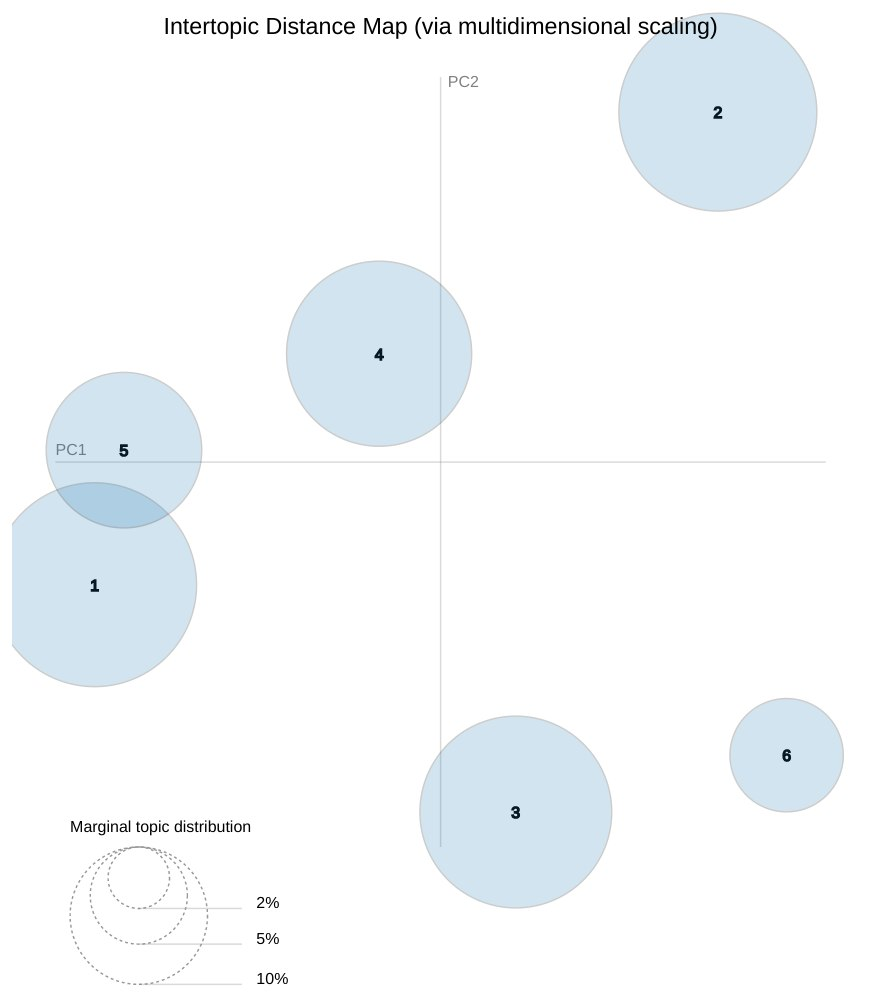
\includegraphics[width=0.45\textwidth]{figures/news_lda.png}
    }
    \hspace{0in}
    \subfigure[游记攻略]{
        \label{travellda}
        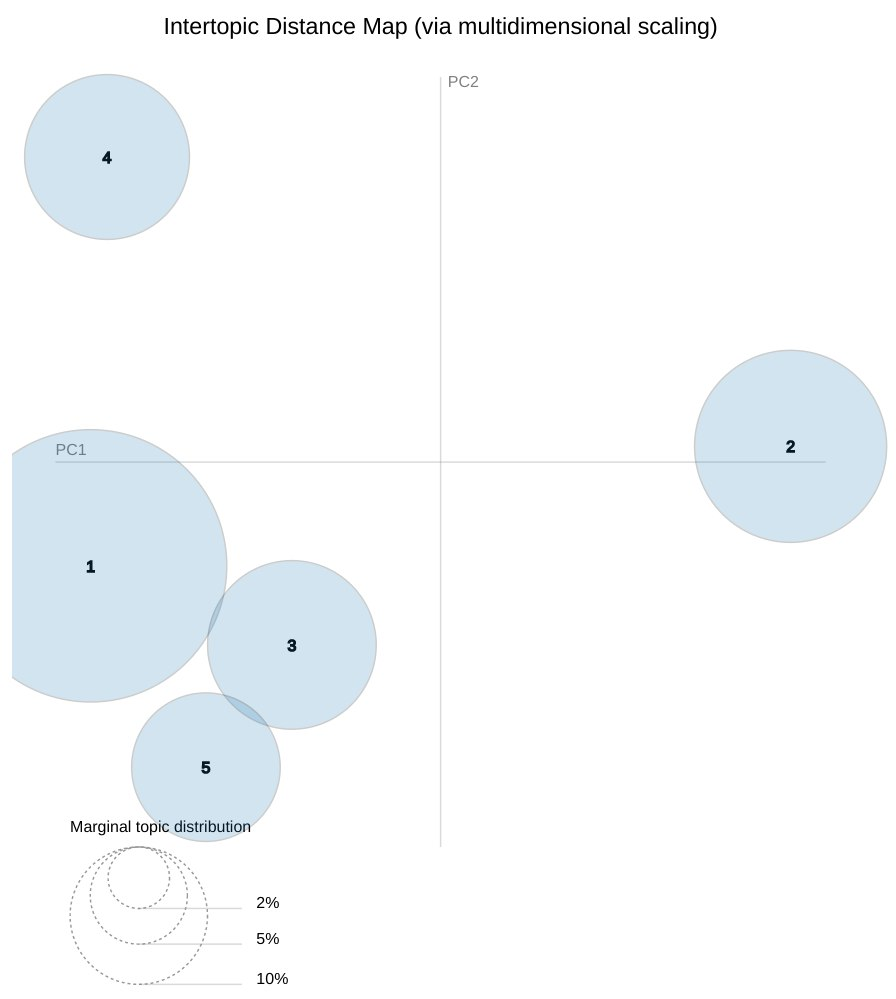
\includegraphics[width=0.45\textwidth]{figures/travel_lda.png}
    }
    \caption{基于LDA模型的文本主题分类}
    \label{lda_fenlei}
\end{figure}

为了验证分类后每个分类与文旅主题词库的匹配程度,本文首先需要对每类文本中的高频词汇进行统计。

对于公众号推文,本文发现,在超参数$K=6$,$\gamma=0$的时候,分类的效果较为理想,经过初步可视化,以其中四个分类的高频词为例,如图\ref{news1}、\ref{news2}、\ref{news3}及\ref{news4}所示:


\begin{figure}[H]
	\centering
	\begin{minipage}{0.49\linewidth}
		\centering
		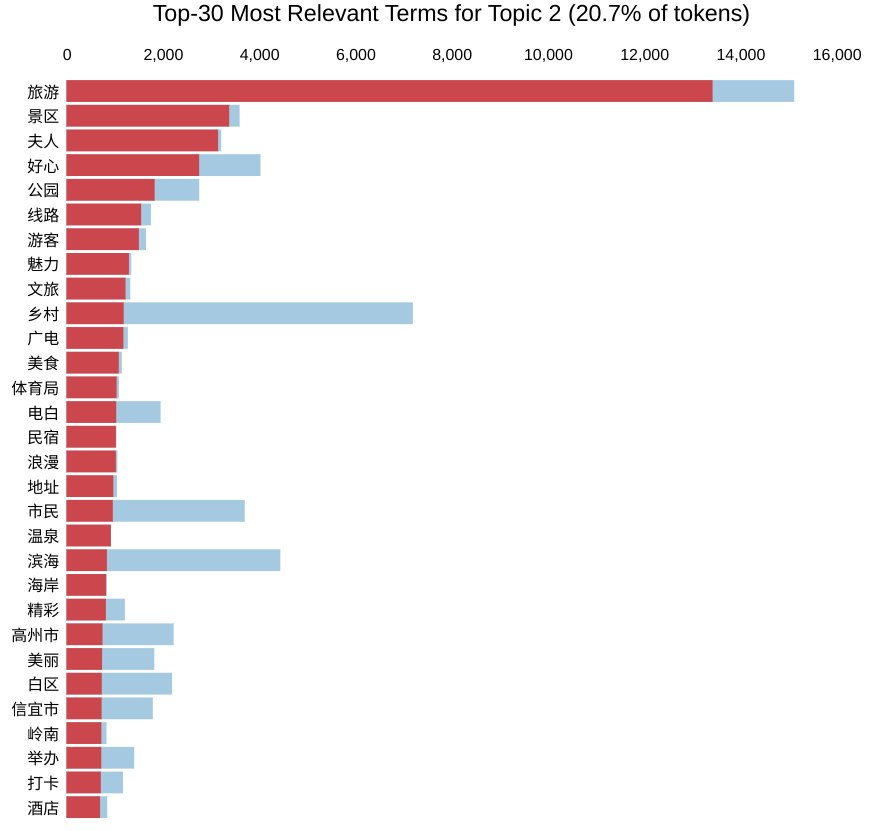
\includegraphics[width=0.9\linewidth]{figures/news1.png}
		\caption{分类2}
		\label{news1}%文中引用该图片代号
	\end{minipage}
	\begin{minipage}{0.49\linewidth}
		\centering
		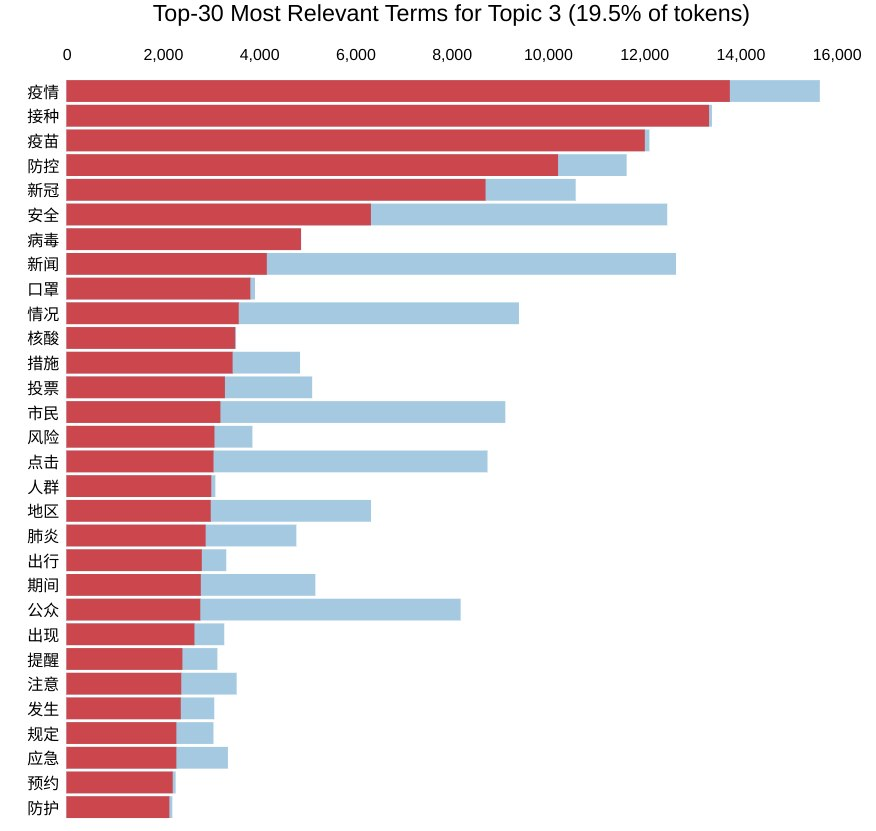
\includegraphics[width=0.9\linewidth]{figures/news2.png}
		\caption{分类3}
		\label{news2}%文中引用该图片代号
	\end{minipage}
	%\qquad
	%让图片换行,
	
	\begin{minipage}{0.49\linewidth}
		\centering
		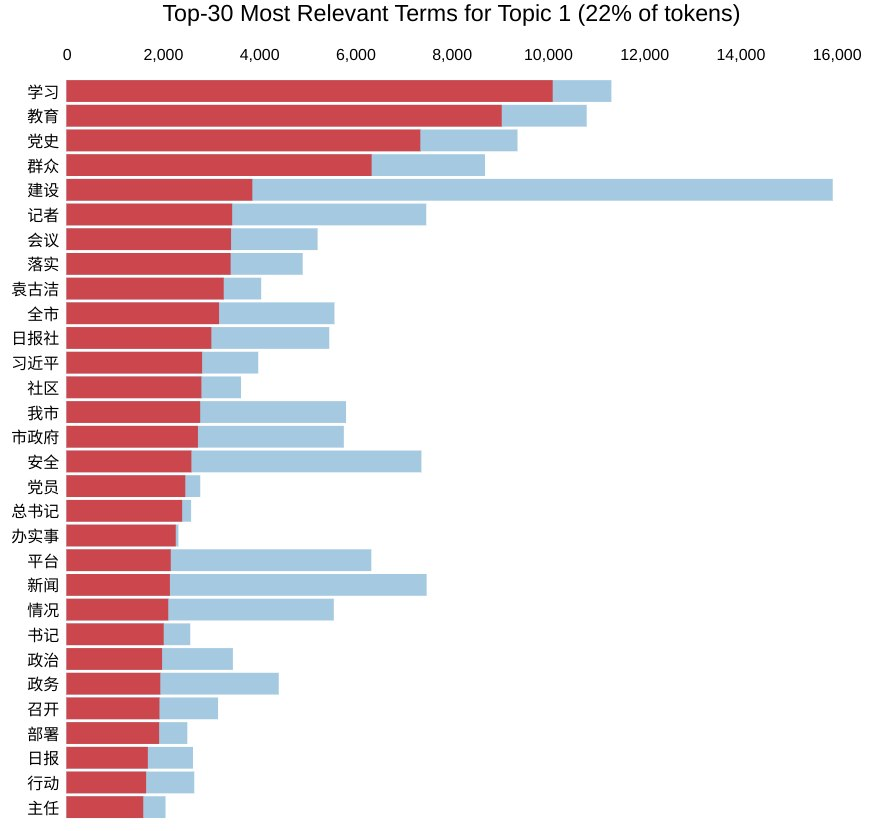
\includegraphics[width=0.9\linewidth]{figures/news3.png}
		\caption{分类1}
		\label{news3}%文中引用该图片代号
	\end{minipage}
	\begin{minipage}{0.49\linewidth}
		\centering
		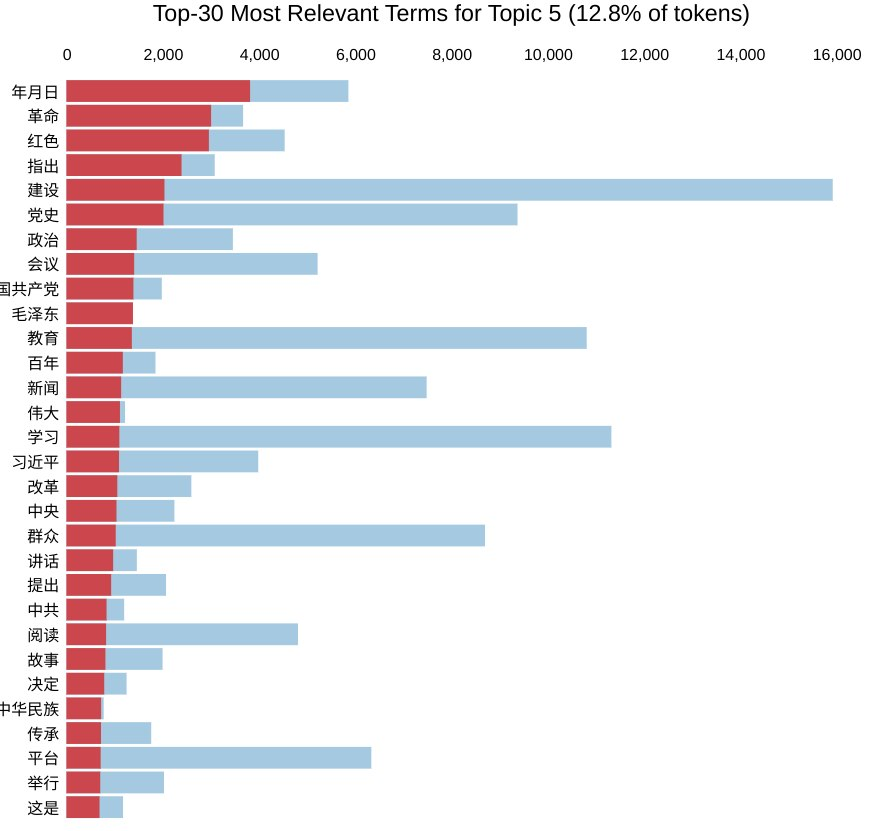
\includegraphics[width=0.9\linewidth]{figures/news4.png}
		\caption{分类5}
		\label{news4}%文中引用该图片代号
	\end{minipage}
\end{figure}

经过初步观察,基于LDA的建模是有效的,图\ref{news1}中展示的分类2的公众号推文高频词汇,其中大多都与文旅主题相关,而图\ref{news2}中显示分类3中的推文基本与疫情相关,图\ref{news2}中显示分类1和5中的推文则与党建、政府工作相关性较大。

对于旅游攻略,本文发现,在超参数$K=5$,$\gamma=0$的时候,分类的效果较为理想,经过初步可视化,以其中两个分类的高频词为例,如图\ref{travel_cipin}所示:

\begin{figure}[H]
    \centering
    \subfigure[分类1]{
        \label{travel1}
        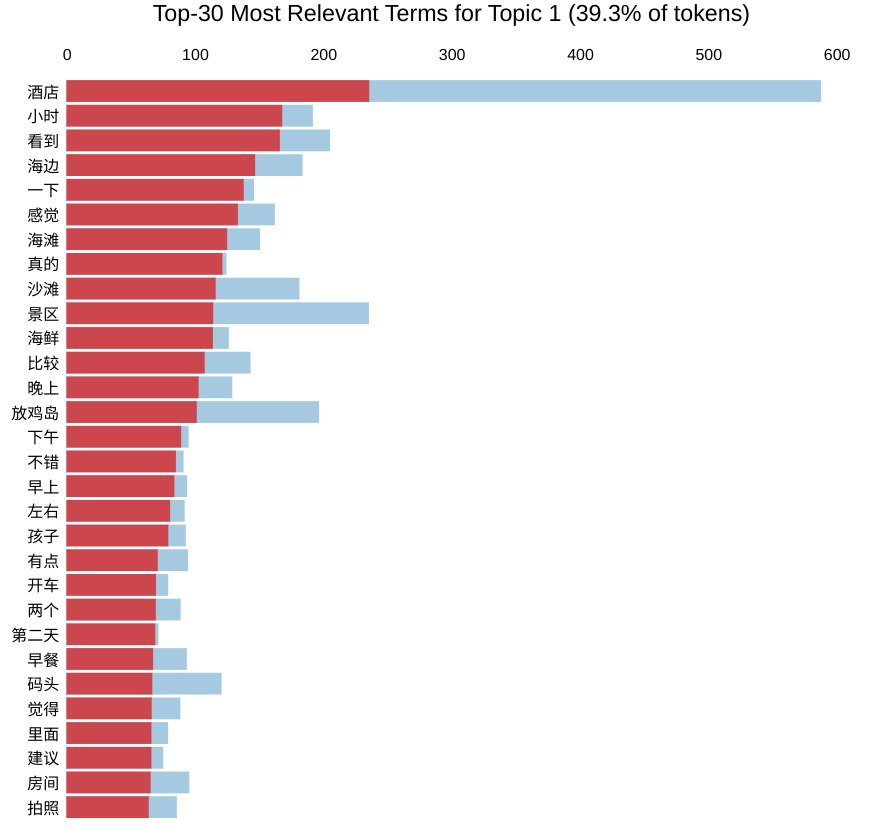
\includegraphics[width=0.45\textwidth]{figures/travel1.png}
    }
    \hspace{0in}
    \subfigure[分类2]{
        \label{travel2}
        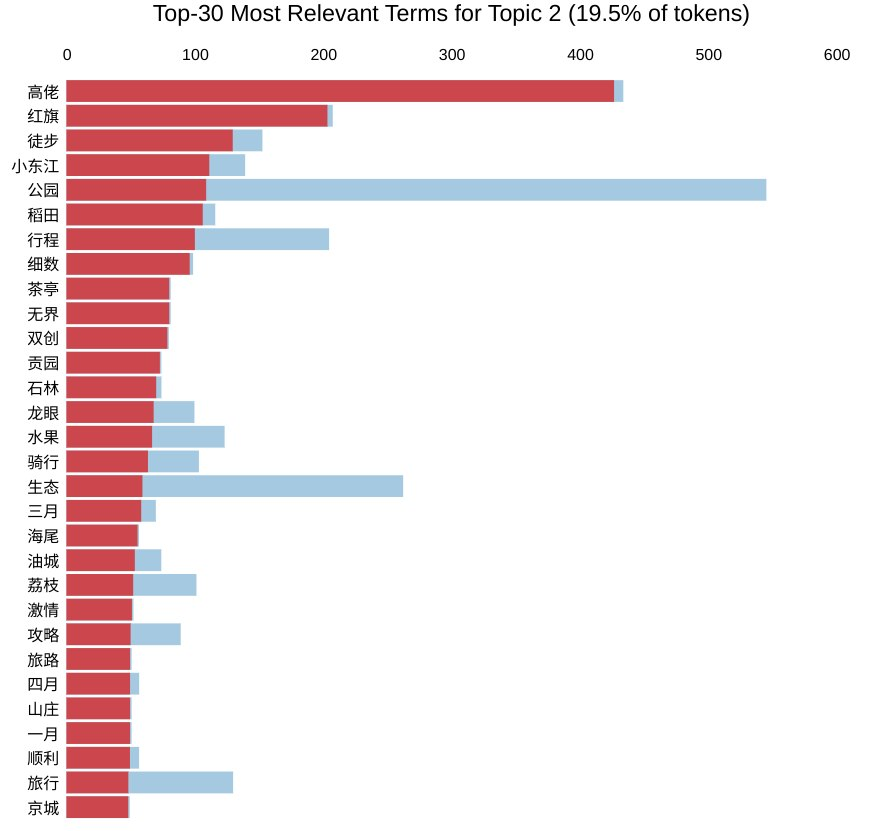
\includegraphics[width=0.45\textwidth]{figures/travel2.png}
    }
    \caption{基于LDA模型的旅游攻略词频分析}
    \label{travel_cipin}
\end{figure}

通过图\ref{travel_cipin}能够看出,LDA主题模型的分类对于旅游攻略文本同样是有效的,文旅相关的文本与党建、团建等无关主题的文本被有效提取了出来。根据上述LDA主题模型的分类结果分析,能够看出该模型对于文本的分类还是较为清晰的,至于文旅主题相关性的判别,本文根据每类文本中高频词与主题词库中高频词的匹配程度对文本进行相关性预测。根据阈值$\gamma$,本文首先选取LDA主题分类中与文旅主题相关的类,该类下的所有样本都被视作与文旅主题相关。相应的,若主题匪类的高频词与主题词库的匹配程度如果低于阈值$\gamma$,则该类中的所有样本都被视作与文旅主题无关。

下表给出了微信公众号推文和游记攻略与文旅主题相关性的判断:

\begin{center}
    \begin{longtable}{c|c|c}
      \caption{微信公众号推文及游记攻略与文旅主题相关性预测}
      \label{wx_yj_related}\\
        \hline
        \textbf{文本类别} & \textbf{相关性} & \textbf{ID(由小到大排序)} \\
        \hline
          公众号推文 & \begin{tabular}[c]{@{}c@{}}
            相关 \\ 不相关 
          \end{tabular} 
          & \begin{tabular}[c]{@{}l@{}}
            1001,1004,1006,1008,……,7267,7269,7281,7284 \\ 1002,1003,1005,1007,……,7282,7283,7285,7286
          \end{tabular} \\
		  游记攻略 & \begin{tabular}[c]{@{}c@{}}
            相关 \\ 不相关 
          \end{tabular} 
          & \begin{tabular}[c]{@{}l@{}}
            1001,1003,1004,1006,……,1291,1292,1293,1294 \\ 1002,1005,1007,1020,……,1211,1251,1254,1266
          \end{tabular} \\
        \hline
    \end{longtable}
    \end{center}

\section{问题二建模与求解}

\subsection{模型的构建与求解}
本问第一步需要从提供的OTA、UGC数据中提取出旅游产品。分析数据可得在酒店、景区和餐饮的数据中分别给出了酒店名称、景区名称和餐饮名称,在游记攻略和微信公众号推文中并未直接给出相关的旅游产品名称。经过观察发现,在这两者的标题和正文中包含了相关的旅游产品名称。因此,需要从这些信息中提取出相关的旅游产品名称。经过分析可以采用命名实体识别(Named Entity Recognition,简称NER) 来从海量文本中提取出我们需要的旅游产品名称。NER是指识别文本中具有特定意义的词(实体),主要包括人名、地名、机构名、专有名词等等,并把我们需要识别的词在文本序列中标注出来。本文采用bert模型来进行NER。本文采取无监督的方式进行NER。首先将已有的权重对bert模型进行初始化,然后将第一问过滤掉不相关后所剩余的相关评论输入模型,提取出相关的旅游产品名称。

下表给出了包含语料ID、产品ID、产品名称的提取结果。
\begin{center}
  \begin{longtable}{c|c|c}
    \caption{旅游产品提取表}
    \label{wx_yj_related}\\
      \hline
      \textbf{语料ID} & \textbf{产品ID} & \textbf{产品名称} \\
      \hline
      酒店评论-1001 & \begin{tabular}[c]{@{}c@{}}
        ID1
        \end{tabular} 
        & \begin{tabular}[c]{@{}l@{}}
          茂名君悦商务酒店
        \end{tabular} \\
        ... & \begin{tabular}[c]{@{}c@{}}
          ...
        \end{tabular} 
        & \begin{tabular}[c]{@{}l@{}}
          ...
        \end{tabular} \\
        景区评论-1001 & \begin{tabular}[c]{@{}c@{}}
          ID90
          \end{tabular} 
          & \begin{tabular}[c]{@{}l@{}}
            中国第一滩旅游度假区
          \end{tabular} \\
          ... & \begin{tabular}[c]{@{}c@{}}
            ...
          \end{tabular} 
          & \begin{tabular}[c]{@{}l@{}}
            ...
          \end{tabular} \\
          旅游攻略-1001 & \begin{tabular}[c]{@{}c@{}}
            ID203
            \end{tabular} 
            & \begin{tabular}[c]{@{}l@{}}
              放鸡岛
            \end{tabular} \\
            ... & \begin{tabular}[c]{@{}c@{}}
              ...
            \end{tabular} 
            & \begin{tabular}[c]{@{}l@{}}
              ...
            \end{tabular} \\
            餐饮评论-1001 & \begin{tabular}[c]{@{}c@{}}
              ID339
              \end{tabular} 
              & \begin{tabular}[c]{@{}l@{}}
                盛香烧鹅(东方市场店)
              \end{tabular} \\
              ... & \begin{tabular}[c]{@{}c@{}}
                ...
              \end{tabular} 
              & \begin{tabular}[c]{@{}l@{}}
                ...
              \end{tabular} \\
              微信公共号文章-1006 & \begin{tabular}[c]{@{}c@{}}
                ID418
                \end{tabular} 
                & \begin{tabular}[c]{@{}l@{}}
                  厦门
                \end{tabular} \\
                ... & \begin{tabular}[c]{@{}c@{}}
                  ...
                \end{tabular} 
                & \begin{tabular}[c]{@{}l@{}}
                  ...
                \end{tabular} \\
      \hline
  \end{longtable}
  \end{center}

  本问第二步需要对旅游产品按年度进行热度分析。分析数据可以得出,本文决定从两点进行热度分析。首先是对评论文本进行情感分析,从消费者对该旅游产品的评论得出该旅游产品是否受大众喜爱。其次,该旅游产品的消费频次也是一个很重要的影响因素。从这两个点出发,本文首先需要对每一个旅游产品的评论进行情感分析。经过分析,本文选用bert模型对文本进行正向和负向的情感分析。最终模型会返回两个处于0到1之间的数。前者大说明该文本为负向情感,并将这个数取负作为该文本的情感得分;后者大的话,说明该文本是正向情感,并将这个数作为该文本的情感得分。其次需要按年统计出每一个产品消费的频次。最终将情感得分和产品消费的频次作为评价该旅游产品热度的依据。本文认为用户对该旅游产品的情感得分在评价该旅游产品热度中更为重要,因此会给情感得分更大的比重。同时因为年份越大,它的热度会比年份小的大。所以本文会提高年份大的旅游产品的得分。最终将所得的旅游产品得分进行归一化进行排序。此外在对旅游产品进行产品类型分类时,我们一共给出了七个类,分别是:景区、酒店、特色餐饮、景点、民宿、乡村旅游、文创,根据评论的内容中是否包含这些关键词对旅游产品进行分类。


下表给出了包含产品ID、产品类型、产品名称、产品热度、年份的旅游产品热度分析。

\begin{center}
  \begin{longtable}{c|c|c|c|c}
    \caption{旅游产品的热度}
    \label{wx_yj_related}\\
      \hline
      \textbf{产品ID} & \textbf{产品类型} & \textbf{产品名称} & \textbf{产品热度}& \textbf{年份}\\
      \hline
      ID1 & \begin{tabular}[c]{@{}c@{}}
        特色餐饮
        \end{tabular} 
        & \begin{tabular}[c]{@{}l@{}}
          渔乐码头烤鱼牛蛙晚饭餐厅
        \end{tabular} 
        & \begin{tabular}[c]{@{}c@{}}
          0.0049
          \end{tabular}
          & \begin{tabular}[c]{@{}c@{}}
            2018
            \end{tabular}\\
        ... & \begin{tabular}[c]{@{}c@{}}
          ...
        \end{tabular} 
        & \begin{tabular}[c]{@{}l@{}}
          ...
        \end{tabular} 
        & \begin{tabular}[c]{@{}c@{}}
          ...
        \end{tabular} 
        & \begin{tabular}[c]{@{}c@{}}
          ...
        \end{tabular} \\

        ID236 & \begin{tabular}[c]{@{}c@{}}
          景区
          \end{tabular} 
          & \begin{tabular}[c]{@{}l@{}}
            茂名森林公园
          \end{tabular} 
          & \begin{tabular}[c]{@{}c@{}}
            0.0064
            \end{tabular}
            & \begin{tabular}[c]{@{}c@{}}
              2019
              \end{tabular}\\
          ... & \begin{tabular}[c]{@{}c@{}}
            ...
          \end{tabular} 
          & \begin{tabular}[c]{@{}l@{}}
            ...
          \end{tabular} 
          & \begin{tabular}[c]{@{}c@{}}
            ...
          \end{tabular} 
          & \begin{tabular}[c]{@{}c@{}}
            ...
          \end{tabular} \\

          ID412 & \begin{tabular}[c]{@{}c@{}}
            酒店
            \end{tabular} 
            & \begin{tabular}[c]{@{}l@{}}
              柏曼酒店(茂名大道东汇城店)
            \end{tabular} 
            & \begin{tabular}[c]{@{}c@{}}
              0.0048
              \end{tabular}
              & \begin{tabular}[c]{@{}c@{}}
                2020
                \end{tabular}\\
            ... & \begin{tabular}[c]{@{}c@{}}
              ...
            \end{tabular} 
            & \begin{tabular}[c]{@{}l@{}}
              ...
            \end{tabular} 
            & \begin{tabular}[c]{@{}c@{}}
              ...
            \end{tabular} 
            & \begin{tabular}[c]{@{}c@{}}
              ...
            \end{tabular} \\
            ID633 & \begin{tabular}[c]{@{}c@{}}
              特色餐饮
              \end{tabular} 
              & \begin{tabular}[c]{@{}l@{}}
                友情有意音乐餐厅
              \end{tabular} 
              & \begin{tabular}[c]{@{}c@{}}
                0.0036
                \end{tabular}
                & \begin{tabular}[c]{@{}c@{}}
                  2021
                  \end{tabular}\\
              ... & \begin{tabular}[c]{@{}c@{}}
                ...
              \end{tabular} 
              & \begin{tabular}[c]{@{}l@{}}
                ...
              \end{tabular} 
              & \begin{tabular}[c]{@{}c@{}}
                ...
              \end{tabular} 
              & \begin{tabular}[c]{@{}c@{}}
                ...
              \end{tabular} \\
      \hline
  \end{longtable}
  \end{center}
\section{问题三建模与求解}

\subsection{图卷积神经网络}

图神经网络(GNN)是近年来十分热门的研究课题。在图神经网络中,实体被视作节点,而实体之间的联系被视作连接节点的边。通过利用神经网络优秀的表现能力,结合知识图谱的范式,图神经网络能够充分提取有连接的节点之间的高阶连接信息,进而能够完成一系列如:节点分类、连接预测等任务,常见的GNN模型包括GCN\cite{kipf_gcn_2017},GAN\cite{peter_gan_2017},GraphSage\cite{hamilton_graphsage_2017}等。

\begin{figure}[!h]
\centering
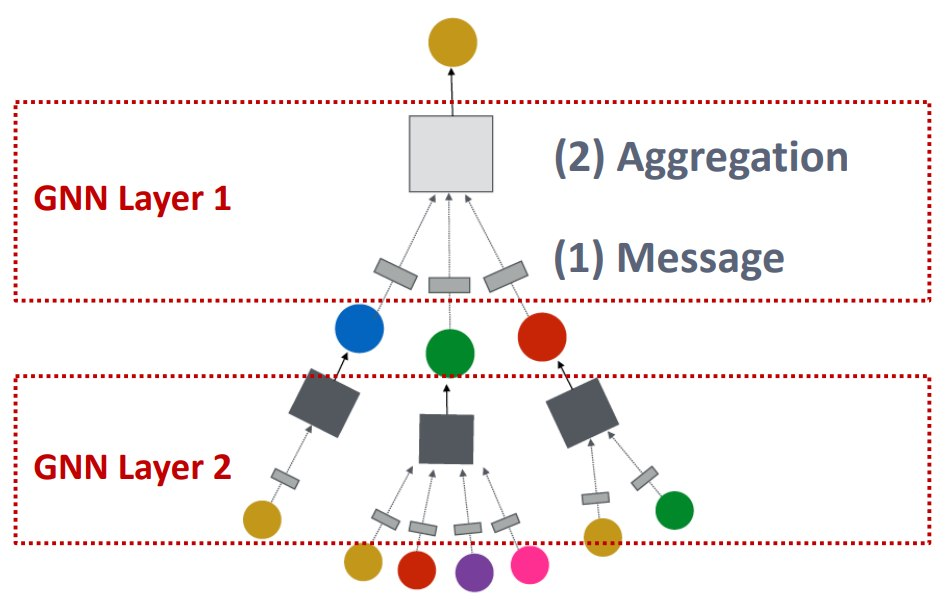
\includegraphics[width=.7\textwidth]{gnn.png}
\caption{图神经网络结构}
\label{gnn}
\end{figure}


图\ref{gnn}给出了图神经网络最重要的表征聚合与信息传递的常见范式。图卷积神经网络(GCN)作为图神经网络的一种,的得名来源于卷积神经网络(CNN)的思想。卷积神经网络是在二维平面对节点做卷积运算,而图神经网络将这一运算拓展至三维空间。GNN中计算最终输出过程中起主要作用的是特征信息聚合与传递。信息传递表现的是节点信息在不同的神经网络层之间的计算,而信息聚合表示的是不同神经网络层之间的节点、连接信息的聚合计算。在信息传递过程中,节点$v$接收来自于每个与其相邻的节点$u$的信息$m_{u}^{(l)}$为:
\begin{equation}
  m_{u}^{(l)} = \frac{W^{(l)}}{|N(v)|}(h_u^{(l-1)}), \ u \in \{N(v) \cup v\}
\end{equation}

其中$W^{(l)}$为可训练的权重参数,$|N(v)|$的引入是为了防止表征在传递与聚合的过程中发生信息在数量级上的变化。

而节点$v$在第$l$层卷积层其自身的表征$h_v^{l}$为:
\begin{gather}
	h_{v}^{(l)} = AGG^{(l)}(\{m_u^{(l)}, u \in N(v), m_v^{(l)}\}), \ u \in \{N(v) \cup v\} \\ 
	= \sigma(\sum \frac{W^{(l)}}{|N(v)|}(h_u^{(l-1)}), \ u \in \{N(v) \cup v\})
\end{gather}

其中$\sigma$为激活函数,$AGG^{(l)}$表示的是聚合函数,在GCN中该函数为和函数。在$l$层神经网络层的传递与聚合后,节点就能够获得其$l-1$阶近邻的信息。

\subsection{模型的构建与求解}

在此问题中,本文的目标是预测节点之间的链接是否存在,其基本思想就是利用图神经网络得到的节点表征预测节点之间链接的可能性得分。对于节点$u$和$v$,其在最后第$L$层的表征分别为$h_u^{L}$与$h_v^{L}$,则两者链接可能性得分可以记为:
\begin{equation}
	y_{u, v} = \phi(h_u^{(L)}, h_v^{(L)})
\end{equation}

模型训练的有效性的评价就包括与节点之间连接性的可能性预测应当大于一个随机噪声分布。在这类问题中,有诸多常用的损失函数,例如:交叉熵损失(InfoNCE)、贝叶斯个性化排序损失(BPR)或是间隔损失等。

本文基于图卷积神经网络(GCN)进行节点间的链路预测。首先,本文根据前文的Bert模型,对每个实体提取了一个768维度的表征,用于刻画该实体的内在特征。由于链接预测是个有监督学习任务,需要根据已有的监督信号,即已有的节点链接进行表征的传递与聚合,进而才能够得到蕴含高阶信息的表征。根据文本在同一篇微信公众号推文或游记攻略中的同时出现情况,则本文认为这两个实体是具备关联的。本文在这里将已有的768维节点表征作为每个节点的初始表征,用于随后的表征的传递与聚合。


\section{问题四建模与求解}

新冠疫情对于旅游行业有重大的影响,最直观的就是短途旅行的增多。显然疫情对于旅游产品实体和实体时间的关联都存在一定影响。本文首先对行业整体在疫情前后的表现进行分析,结果如表\ref{hangye_beforeafter}:

\begin{center}
    \begin{longtable}{c|c|c|c|c}
      \caption{疫情前后旅游行业经营状况}
      \label{hangye_beforeafter}\\
        \hline
        \textbf{文本类别} & \textbf{情感得分(前)} & \textbf{情感得分(后)} & \textbf{消费频率(前)} & \textbf{消费频率(后)} \\
        \hline
          酒店 & 0.069 & 0.089 &  8.34 & 13.69 \\
		  民宿 & 0.084 & 0.032 &  8.67 & 1.33 \\
		  乡村旅游 & 0.081 & 0.076 & 18.00 & 1.00 \\
		  特色餐饮 & 0.064 & 0.065 & 42.04 & 79.55 \\
		  景区 & 0.047 & 0.056 & 5.62 & 6.68 \\
		  景点 & 0.075 & 0.056 & 1.89 & 1.07 \\
        \hline
    \end{longtable}
    \end{center}

针对前文分得的行业在疫情前后的表现来看,出现用户满意度提升的主要体现在酒店方面,能够看出经过疫情后,酒店行业在用户的满意程度上有较为明显的提升。而同为住宿产品的民宿行业却出现用户满意度下滑较大的情况,出现了大幅度的下降。而别的行业从用户满意度而言有增有减。而消费频率发现,酒店和餐饮都有较大的提升,相应的,民宿和乡村旅游有较大的减少。

能够看出,酒店在疫情前后都表现出了较好的复苏情况,而民宿行业却出现了明显的萎缩。由于其两者互为竞争关系,出现这种情况可能源自于酒店因为其自身较为规范的管理和服务,为游客提供了更为稳定的选择。而特色餐饮的热度有所提升,但用户满意度未出不变,这可能是因为近年来越来越多的商家开始利用OTA和UCG信息进行产品推广和品牌营销导致的。而乡村旅游的热度出现了较大跌幅,经过观察是因为一特定商家的变化导致的。

随后本文对在疫情前后消费频率较高的旅游产品进行排序,发现其中最热门的产品基本都是特色餐饮产品,出现了许多餐饮产品翻倍级别的增长。而其余旅游产品的表现则较为平稳。这其中的原因很有可能是因为疫情后许多餐饮商家更加重视通过OTA和UCG信息进行营销。

%参考文献   手工录入
%\begin{thebibliography}{9}%宽度9
% \bibitem{bib:one} ....
% \bibitem{bib:two} ....
%\end{thebibliography}


\bibliographystyle{gmcm}
\bibliography{example}


% \newpage
% %附录
% \appendix
% %\setcounter{page}{1} %如果需要可以自行重置页码。
% \section{我的 MATLAB 源程序}
% \begin{lstlisting}[language=Matlab]%设置不同语言即可。
% kk=2;[mdd,ndd]=size(dd);
% while ~isempty(V)
% [tmpd,j]=min(W(i,V));tmpj=V(j);
% for k=2:ndd
% [tmp1,jj]=min(dd(1,k)+W(dd(2,k),V));
% tmp2=V(jj);tt(k-1,:)=[tmp1,tmp2,jj];
% end
% tmp=[tmpd,tmpj,j;tt];[tmp3,tmp4]=min(tmp(:,1));
% if tmp3==tmpd, ss(1:2,kk)=[i;tmp(tmp4,2)];
% else,tmp5=find(ss(:,tmp4)~=0);tmp6=length(tmp5);
% if dd(2,tmp4)==ss(tmp6,tmp4)
% ss(1:tmp6+1,kk)=[ss(tmp5,tmp4);tmp(tmp4,2)];
% else, ss(1:3,kk)=[i;dd(2,tmp4);tmp(tmp4,2)];
% end;end
% dd=[dd,[tmp3;tmp(tmp4,2)]];V(tmp(tmp4,3))=[];
% [mdd,ndd]=size(dd);kk=kk+1;
% end; S=ss; D=dd(1,:);


%  \end{lstlisting}


\end{document} 